\documentclass[12,twoside]{mammeTFM}
%\usepackage[active]{srcltx}
\usepackage{amsthm} % To make environments with different styles.
\usepackage{amsmath,amssymb,amsfonts} % Multiple mathematics symbols and fonts.
%\usepackage{amscd} % To make commutative diagrams
\usepackage{graphicx} % To include figures in a simple way. Fancy options can be found for example in http://www.kwasan.kyoto-u.ac.jp/solarb6/usinggraphicx.pdf
\usepackage{enumerate} % It allows you to make list with specific somehow arbitrary labels, like this one.
%\usepackage[all]{xy} % To make really fancy commutative diagrams
\usepackage{booktabs} % To make fancy tables.
%\usepackage[usenames]{xcolor}
%\usepackage{fancyhdr}

%%%%% My packages (Should probably push all the header to a certain file and include it in each latex.

%\usepackage[left=15mm, right=15mm]{geometry}
\usepackage[utf8]{inputenc}
\usepackage[english]{babel}
\usepackage{bigfoot}
%\usepackage{algorithm}
%\usepackage[noend]{algpseudocode}
\usepackage{epstopdf}
\usepackage{vhistory}
\usepackage{framed}
\usepackage{hyperref}
\usepackage{cancel}
\usepackage{subcaption}

\setlength{\parskip}{11pt}

% Theorem Environments: add extra ones at the end if you need it.
\newtheorem*{thmA}{Theorem A}
\newtheorem{thm}{Theorem}[section]

\newtheorem{prop}[thm]{Proposition}
\newtheorem{lem}[thm]{Lemma}
\newtheorem{cor}[thm]{Corollary}
\newtheorem{conj}[thm]{Conjecture}

\theoremstyle{definition}
\newtheorem{definition}[thm]{Definition}
\newtheorem{exmp}[thm]{Example}

\theoremstyle{remark}
\newtheorem{remark}[thm]{Remark}
\newtheorem*{remarknonumber}{Remark}
\newtheorem{observation}[thm]{Observation}
%%% My own theorems
\newtheorem{main_thm}[thm]{Main Theorem}

%% rme, rmi e Id son el número e, el número imaginario i y la identidad respectivamente. Poned ds antes de una expresión
%% cuando salga mal (en las fracciones y cosas parecidas)
\def\ds{\displaystyle}
\def\rme{\mathrm{e}}
\def\rmi{\mathrm{i}}
\def\Id{\mathrm{Id}}
\def\resposta{\bullet\bullet\bullet\bullet\bullet\bullet}

%%%%%%%%%%%%%%%%%%
% macros/abbreviations: Include here your own.
%%%%%%%%%%%%%%%%%%

%% Conjuntos típicos.
\newcommand{\N}{\ensuremath{\mathbb{N}}}
\newcommand{\E}{\ensuremath{\mathbb{E}}}
\newcommand{\Z}{\ensuremath{\mathbb{Z}}}
\newcommand{\Q}{\ensuremath{\mathbb{Q}}}
\newcommand{\R}{\ensuremath{\mathbb{R}}}
\newcommand{\C}{\ensuremath{\mathbb{C}}}
\newcommand{\F}{\ensuremath{\mathbb{F}}}
\newcommand{\MP}{\ensuremath{\mathbb{P}}}

% math stuff
\newcommand{\Expect}{\ensuremath{{\rm I\kern-.3em E}}}
\newcommand{\Var}{\ensuremath{\mathrm{Var}}}
\newcommand{\Cov}{\ensuremath{\mathrm{Cov}}}

% random
\makeatletter
\newcommand{\raisemath}[1]{\mathpalette{\raisem@th{#1}}}
\newcommand{\raisem@th}[3]{\raisebox{#1}{$#2#3$}}
\makeatother

\newcommand{\function}[5]{\begin{align*} #1\colon #2 &\to #3 \\ #4 &\mapsto #5\end{align*}}
\newcommand{\vega}{\nu}

%% Separacio correcta paraules final de linia.
\hyphenation{Bar-ce-lo-na}

%% Ejemplo de como hacer una tabla.

%\begin{tabular}{|r|c|c|}
%\hline
%$n$	&nº bits (estándar)	&nº bits (\emph{sp. triplet})\\
%\hline
%10   	  &  6400       	& 3040\\
%\hline
%50   	  & 160000    	& 78400\\
%\hline
%100 	  & 640000    	& 314320\\
%\hline
%200 	  & 2560000  	& 1262320\\
%\hline
%400 	  & 10240000	&5043680\\
%\hline
%650 	  & 27040000	&13282720\\
%\hline
%1000 	  & 64000000	&31479040\\
%\hline
%\end{tabular}


%% Ejemplo de como hacer una figura

%\begin{figure}[ht]
%\centering
%\includegraphics[width=6cm,angle=-90]{exemple.eps}
%\caption{Corba de continuaci\'o d'$u_2$ com a funci\'o de $\lambda$.}
%\label{fig:etiqueta}
%\end{figure} 

%% se puede hacer \input{archivo.tex} en lugar de \includegraphics

%% Y de como hacerle referencia

% bla bla bla en la Figura~\ref{fig:etiqueta}


% Body of document

\titol{This is the long title\\[3mm] with a line skip}
\titolcurt{Heston Calibration using SWIFT}
\authorStudent{Eudald Romo Grau}
\supervisors{(name of the supervisor/s of the master's thesis)}
\monthYear{Month, year}

%\msc[2010]{Primary  	55M25, 57P10, Secondary 55P15, 57R19, 57N15.}

\paraulesclau{Derivatives Trading, Heston, SWIFT, calibration}
\agraiments{
Thanks to...}


\abstracteng{This should be an abstract in English, up to 1000 characters.}

%%%%%%%%%
\begin{document}

\maketitle

\tableofcontents

\pagebreak

% The expected structure is explained in https://bibliotecnica.upc.edu/estudiants/6-passos-que-teu-tfg/tfm-sigui-exit/escric-meu-tfg/tfm#criteris-grafics

\section{Motivation}

Option pricing has an important role in contract trading, both as a form of derivative trading in itself, as a way to hedge other stock or derivative portfolios.

Pricing these options can have a broad range of difficulty, mainly due to two factors:
\begin{enumerate}[\bf (1)]
\item {\tt Contract type: } These options can take a variety of forms, from the vanilla European Options to more complex American or Asian options (TODO: citations).
\item {Underlying Model: } The price of the derivative depends on the future price of its underlying. The evolution of this price can be modeled using simpler models like Black \& Scholes, or using other models that take into account more theoretical results related to the underlying price evolution, like the Heston model. {TODO: citations, add more models.}
\end{enumerate}

There are only closed analytic solutions for the Option pricing problem for the simpler contracts and models: European options under BS and can have no analytic solution when one either trades a more complicated contract (like American options) or uses a more complex model (like Heston) to model its dynamics.

The advantages of simpler models tend to be faster computations and possibly analytic functions to compute the price. On the other hand, they fail to capture more complex behavior of the market.

For example, BS is probably the most used model in real option trading (TODO: back this up) but fails to capture the well-known high kurtosis and negative skewness of the log returns volatility, which motivated the development of the Heston model, which will be the center of this study.

Most of these models can be used to price different strikes using a set of intrinsic parameters. Usually this parameters are calibrated either using historical data or using data from options with the same underlying at different strikes and, sometimes, different maturities. (TODO: Cite) In the second calibration mode, which is usually used in the trading world, particularly in high frequency trading, (TODO: cite) fast option calculation methods and model calibration techniques are required to be able to update the model in real time.

In particular, solving the Heston model calibration is a difficult optimization problem to solve, partly due to it being a multidimensional optimization problem with a mainly unknown structure: it is not known whether it is a convex problem or not nor whether it generally has a single solution or not. Because of that, several different branches of research have appeared, but they are either deterministic but slow, or use heuristics or assumptions about the model parameters to reduce the dimension of the problem.

A branch of numerical option pricing that, given a density function (and the value of its parameters) to describe the stochastic evolution of the underlying over time, use its characteristic function to valuate the price of the option with different strikes and maturities.

Traditionally, using this pricing method combined with a gradient-descent based method for calibration was not possible due to the characteristic function derivatives with respect of the model parameters being too intractable.

Recently, there has been both work in fast option pricing numerical techniques using characteristic functions (TODO: cite) and giving simple expressions for the characteristic function (TODO: cite) of the Heston model (its previous expressions either had complex variable discontinuities that translated in numeric problems (TODO: cite) or complicated derivative expressions, which made it difficult to use in gradient descent based methods).

This work is centered around the calibration of the Heston model for European Options (choosing proper values of the model parameters to minimize the option valuation error) by using a gradient descent method (TODO: name properly) valuating the option and its partial derivatives using the new characteristic function approach in the SWIFT setup.

\section{Nomenclature}

I will probably not add this section (that's why it doesn't have fancy formatting), but it's good to have everything set recorded somewhere and I might finally decide to polish it up and include this section.

$t$ will refer to the time at which the option is being valuated

$T$ will be the expiration time. Given a time-dependent variable $Var$, $Var_t$ will refer to the value of that variable at time $t$ (respectively with $T$). 

$\tau := T - t$

$S, K$ will refer to the underlying and the strike prices respectively.

$r$ will refer to the risk-free interest rate.

$q$ will refer to the discount rate.

\section{Option Valuation}

\begin{definition}
An European Option is a derivative contract on an underlying asset that fixes a transaction price (called \textbf{strike price}), an expiration time (also called \textbf{maturity}), and an \textbf{underlying} asset quantity and gives the holder of the contract the right (but not the obligation) of buying (Call Option) or selling (Put Option) the specified quantity of the underlying at the Strike price on expiration.
\end{definition}

In the following sections we will use the following nomenclature for Option parameters: $t$ will refer to the time at which the option is being valuated and $T$ will be the expiration time. Given a time-dependent variable $V$, $V_t$ will refer to the value of that variable at time $t$ (respectively with $T$). $S, K$ will refer to the underlying and the strike prices respectively.

Slight variations of these terms can give rise to other families of options by facilitating the exercising of the contracts, like the Bermudan and American options (which allow to exercise your buying/selling right at specified instants of time or at any point prior to expiry, respectively).

Other groups of option families are obtained by changing the definition of the option payoff, that is, the amount of money (be it in cash or in the value of the underlying obtained) the option gives on expiration.

\begin{definition} Payoff of a Call European option:
\begin{equation}
V_{EC}(S_T, 0) = (S_T - K)\boldsymbol{1}_{S_T \geq K} = \left\{ \begin{array}{rcl}
S_T - K & \mbox{if} & S_T > K \\ 
0 & \mbox{if} & S_T\leq K
\end{array}\right.
\end{equation} 
\end{definition}

So, on maturity, a European Call option is only profitable if it allows the holder of the contract to buy the underlying asset at a cheaper price than the current asset spot price. In most models any option has a certain positive value if it's not expired, as the underlying price can always theoretically move enough so that a currently non-profitable option ends up with a positive payoff on expiry. Another 

\begin{definition} A Call European option at time $t$ is called:
\begin{itemize}
\item {Out of the money (OTM):} If $K > S_t$ (that is, it has no value apart from time value).
\item {At the money (ATM):} If $K = S_t$ (the price of a real option contract will rarely match perfectly the underlying asset price, but one can refer to a theoretic ATM option, for example to describe a volatility surface).
\item {In the money (ITM):} If $K < S_t$ (that is, even if it were to expire right now, it would still hold some implicit value).
\end{itemize}

\end{definition}

Some examples of other families of functions that have different payoffs are Binary Options (only have two possible payoffs dependent on $K$ and $S_T$) and Asian Options (the payoff depends on the mean price of the underlying since the start of the contract and until maturity).

In order to price an option that expires at some point in the future, one usually first models the temporal evolution of the price of its underlying asset by using some stochastic process. This model will typically be expressed in terms of parameters that will be calibrated to fit the underlying price evolution of each product one wants to valuate.
% TODO: Some discussion on how the nature of the contract affects the difficulty of pricing it.

\subsection{No arbitrage and risk neutrality assumptions.}

Put-Call parity (that's why we only talk about Calls in this article)

Model Log-Returns = $\dfrac{log(S_T)}{S_t}$

\subsection{European Option Valuation} \label{subsec:european_option_valuation}
The payoff of some option contracts, like Bermudan, Asian or American options, depends on the price of the underlying asset at several points in time, or even through all its life. European options payoff, on the other hand, only depends on the final price of the underlying asset on the moment of expiration of the contract ($S_T$). 

A general pricing formula for this kind of options uses risk neutrality to compute the option price as the discounted expectation of the payoff at expiry. Then the pricing problem converts to obtaining an stochastic process describing $S_T$ conditioned to the initial value $S_t$. If one considers generic stochastic variables x and y that fully describe the stochastic variables $S_t$ and $S_T$ respectively, the general pricing formula becomes:
\begin{equation}
\label{eq:integral_option_valuation}
v(x, \tau)  = e^{-r \tau}\E^{\Q}(v(y, 0)|x)  = e^{-r\tau} \int_{\R}v(y,0)f(y|x)dy)
\end{equation}
, where v denotes the option value, r the risk-neutral interest rate, $\E^Q$ the expectation under the risk-neutral measure.

Any choice of x and y will allow computing the value of the option through a numerical integration scheme, but most common underlying price models used for option pricing have simpler expressions in the log space, so a common choice when solving this expression is to define:
\begin{align}
\label{eq:y}
y = ln \left(\dfrac{S_T}{K} \right) \\
\label{eq:x}
x = ln \left(\dfrac{S_t}{K} \right)
\end{align}

Given this maturity state variable choice, one can express the payoff of a European put option as
\begin{equation} \label{eq:european_payoff}
v_{K}(y, 0) := K \cdot (1 - e^y)^{+} := K \cdot max(1 - e^y, 0)
\end{equation}
This expression has a lineal dependency with the strike of the option, so one can define the strike-free payoff:
\begin{equation}
g(y) := (1 - e^y)^{+} = \dfrac{v_{K}(y, 0)}{K}
\end{equation}

\begin{remark}
When solving equation \ref{eq:integral_option_valuation} using numerical methods, one should prefer calculating the price of a call option via the price of a put one with the same strike and apply the put-call parity formula to recover the original call price, as $e^y$ can have arbitrarily large values inside the integration domain which can lead to errors due to floating point arithmetics \cite{mar17}.
\end{remark}

There is a broad literature in methods to solve this integration problem for basic underlying asset models. Some of them, as Black and Scholes (BS), even have closed solutions (as will be seen in section \ref{subsec:bs}) but it is common that, for more complex models, $f(y|x)$ doesn't have a known expression.

In some cases, this can be circumvented by using numerical integration methods based on Fourier transforms, if there is a known expression for the characteristic function of $f(y|x)$
\begin{equation}
\hat{f}_y(u;x) = \int_{\R} f(y | x) e^{-iux} du
\end{equation}

This is the case of the L\'evi models and the Heston model which will be presented in the following sections.

\section{L\'evy Processes}
Some well known underlying asset log returns theoretical stochastic processes, as the Geometric Brownian Motion (GBM) model (known as the Black-Scholes-Merton\cite{bs73, mer73} model), can be considered inside a more general concept called L\'evy processes.

\begin{definition} A stochastic process $X = \{X_t : t \geq 0\}$ is considered a L\'evy process if:
\begin{itemize}
\item $X_0 = 0$ almost surely.
\item For any $0 \leq t_1 \leq t_2 \leq \cdots \leq t_n \leq \infty$, $X_{t_2} - X_{t_1}, X_{t_3} - X{t_2}, \cdots X{t_n} - X_{t_{n-1}}$ are independent.
\item $\forall s < t$, $X_t - X_s$ is equal in distribution to $X_{t-s}$
\end{itemize}
\end{definition}

A famous property of L\'evy processes is the L\'evy-Khintchine formula:
\begin{lem}\label{levy_khin} Let $X = (X_t)_{t\geq 0}$ be a L\'evy process. Then its characteristic function $Char_X(u)$ is:
$$
Char_X(u)(t) := \E \left[e^{i\theta X(t)}\right] = e^{t\left(aiu - \dfrac{\sigma^2 u^2}{2} + \int_{\{0\}^c}(e^{iu x} \textbf{I}_{|x| < 1})\Pi(dx)\right)} = e^{\psi_L(w)}
$$
, where $\psi_L(u)$ is called the characteristic L\'evy exponent, and $a \in \R$, $\sigma \geq 0$, and $\Pi$ is the L\'evy measure of X, a $\sigma$-finite measure satisfying $\int_{\{0\} ^c}(1 \wedge x^2)\Pi (dx) < \infty$
\end{lem}

Note that any L\'evy process can be completely characterized by the triplet $(a, \sigma, \Pi)$, which represent a linear drift, a Brownian motion, and a L'evy jump process respectively.

L'evy models in option pricing typically consider x and y as in expressions \ref{eq:x} and \ref{eq:y} and let $X_t := x$, $X_T := y$, and model the log returns evolution by a L'evy process. Then $\hat{f}(y|x) = \hat{f}(X_T|X_t)$ can be obtained through formula \ref{levy_khin}:
\begin{equation}\label{eq:levy_char}
\hat{f}_{y}(u; x) := 
\E\left[e^{iu X_T}\right] = 
\E\left[e^{iu (X_t + X_{T-t})}\right] = 
e^{-iu x}e^{-i u \mu_L T + T \psi_L(-u)} = 
e^{-iu x}\hat{f}(u) = 
\hat{f}_{y - x}(u)
\end{equation}

, where $\mu_L:= r - \psi_L(-i)$ is a drift correction term and $\psi_L(u)$is the characteristic L\'evy exponent of the underlying log-returns process.

\subsection{Black-Scholes-Merton Model} \label{subsec:bs}

A particular case of L\'evi processes is the widely used BS model, originally presented in \cite{bs73} by using the following stochastic differential equation:
\begin{definition} BS model price equation:
\begin{equation}
dS_t = \mu S_t + \sigma S_t W_t
\end{equation}
, where $W_t$ is a Brownian Motion process, $\sigma$ is called the BS volatility, and $\mu$ describes the drift of the underlying log returns and is usually considered $\mu = r - q$ for divident-free products.
\end{definition}

This model assumes the underlying process $S_t$ follows a lognormal distribution with standard deviation $\sigma$ and, for European options, equation \ref{eq:integral_option_valuation} can be solved analytically, obtaining the well-known BS valuation formula:

\begin{lem} \textbf{Black-Scholes-Merton valuation formula for European Call Options}:
\begin{align}
  C_K(\sigma; S_t, \tau) &= N(d_1)S_t - N(d_2) PV(K) \\
     d_1 &= \frac{1}{\sigma\sqrt{\tau}}\left[\ln\left(\frac{S_t}{K}\right) + \left(r + \frac{\sigma^2}{2}\right)(\tau)\right] \\
     d_2 &= d_1 - \sigma\sqrt{\tau} \\
PV(K) &=Ke^{-r\tau}
\end{align}
\end{lem}

The characteristic function $\hat{f}(u)$ can be obtained by setting $\psi_L (u) = -\dfrac{\sigma^2}{2}u^2$ in equation \ref{eq:levy_char} resulting in:
\begin{definition} \textbf{BS characteristic function:}
\begin{equation}
\hat{f}_{BS}(u) = exp{\left(-iu \left( r-q - \dfrac{1}{2}\sigma^2 \right) \tau - \dfrac{\sigma^2 u^2 \tau}{2} \right)}
\end{equation}
\end{definition}

\subsection{Implied Volatility smile and surface} \label{subsec:smile_and_surf}
If the GBM process modeled accurately real market prices, the BS model could be calibrated using several strikes to obtain a single implied volatility value, and that value would be a good estimator of the standard deviation of the historical standard deviation of the lognormal distribution of the underlying returns (which is called the historical BS volatility). This volatility could then be used to price any option of a given strike and maturity. 

In real markets, if one chooses a fixed expiry and calibrates a set  m different models using m different strikes $\{K_i\}$, the obtained implied volatilities $\{\sigma_i\}$ will probably differ. Further, if one estimates the historical volatility $\sigma_H$ from the historical log-returns, the obtained value may not coincide with any of the obtained implied volatilities.

If one were to plot the implied $\sigma_i$ over $K_i$, one would obtain a result similar to the ones in Figure \ref{fig:smile}, but the exact shape would depend on the underlying (and change over time). This strike evolution is traditionally called volatily smile (though it can have different names depending on the shape it takes, like volatility skew for equity markets).

There are several justifications as to why such smiles exist. Some of them involve limitations in the GBM description of the underlying stock returns, but some appeared after significant events, like the volatility skew in equity option markets, which only appeared after the stock market crash of 1987 \cite{hul09}. Their significance is better described with the concept of implied distribution.

If one assumes that the risk-neutrality and no-arbritage concepts hold true, then the real market option prices should follow from specifying a distribution function $f(y|x)$ and solving equation \ref{eq:integral_option_valuation}. One can then estimate the shape of the implied distribution $f(y|x)_I$ that would better match the option prices of a specific product and expiry (there are several techniques to do it, some described in \cite{jac96, pea00}). As can be seen in Figure \ref{fig:implied_distribution}, the upward trend in implied volatility for the deep ITM and OTM options in currency markets is translated into the implied distribution having fatter tails, and the upward trend for small strikes in equity markets translates into a distribution with higher stock market crash probabilities.

A similar effect happens when one fixes a strike price and computes its implied volatility over serveral expiries. The shape that results from plotting the implied volatility smile over time is called term structure and, when one plots the implied volatility over both strike price and time, one gets the so-called implied volatility surface.

The shape of the implied volatility surface holds certain information about the historical performances of the underlying. In particular, the distribution with fat tails implied by the currency market option prices describes the historical returns of the options underlying better than the GBM \cite{hul09}. This shows the inedequacies of the GBM model and the need for better theoretic descriptions of the underlying returns.

\begin{figure}
\centering
\begin{subfigure}{.5\textwidth}
  \centering
  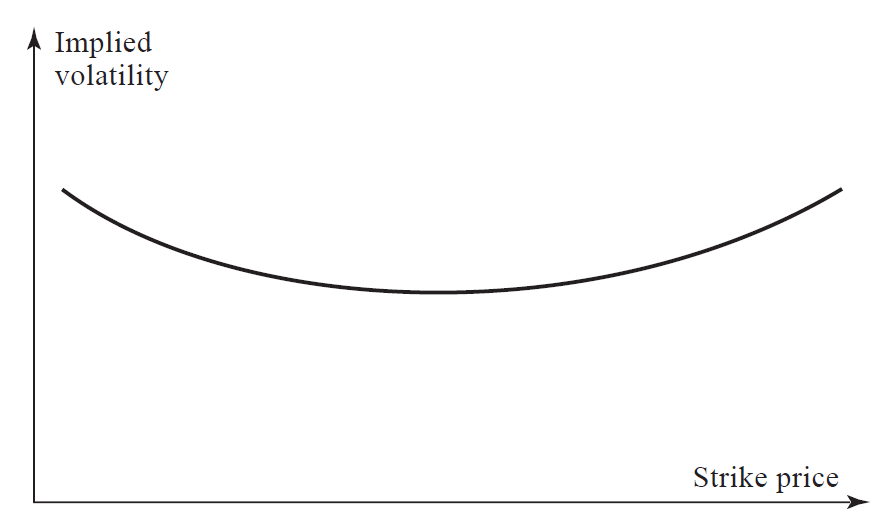
\includegraphics[width=.9\linewidth]{Media/currency_smile.PNG}
  \caption{Foreign Currency market.}
%  \label{fig:sub1}
\end{subfigure}%
\begin{subfigure}{.5\textwidth}
  \centering
  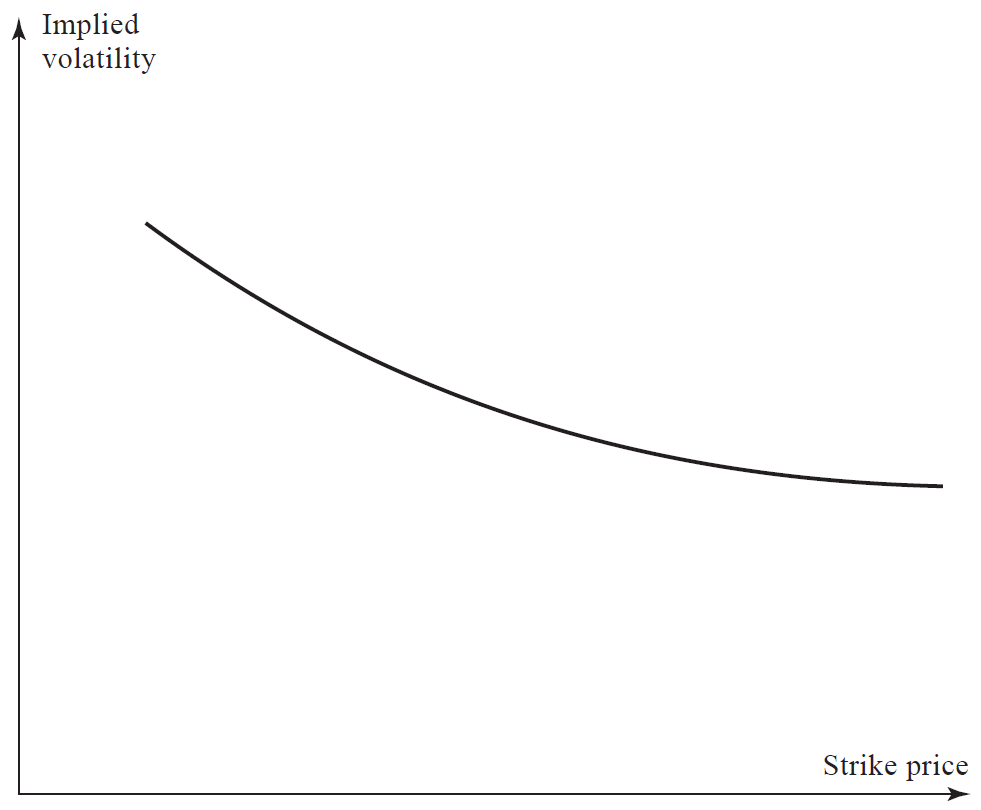
\includegraphics[width=.65\linewidth]{Media/equity_smile.PNG}
  \caption{Equity market.}
%  \label{fig:sub2}
\end{subfigure}
\caption{From \cite{hul09}. Volatility smiles for typical markets.}
\label{fig:smile}
\end{figure}


\begin{figure}
\centering
\begin{subfigure}{.5\textwidth}
  \centering
  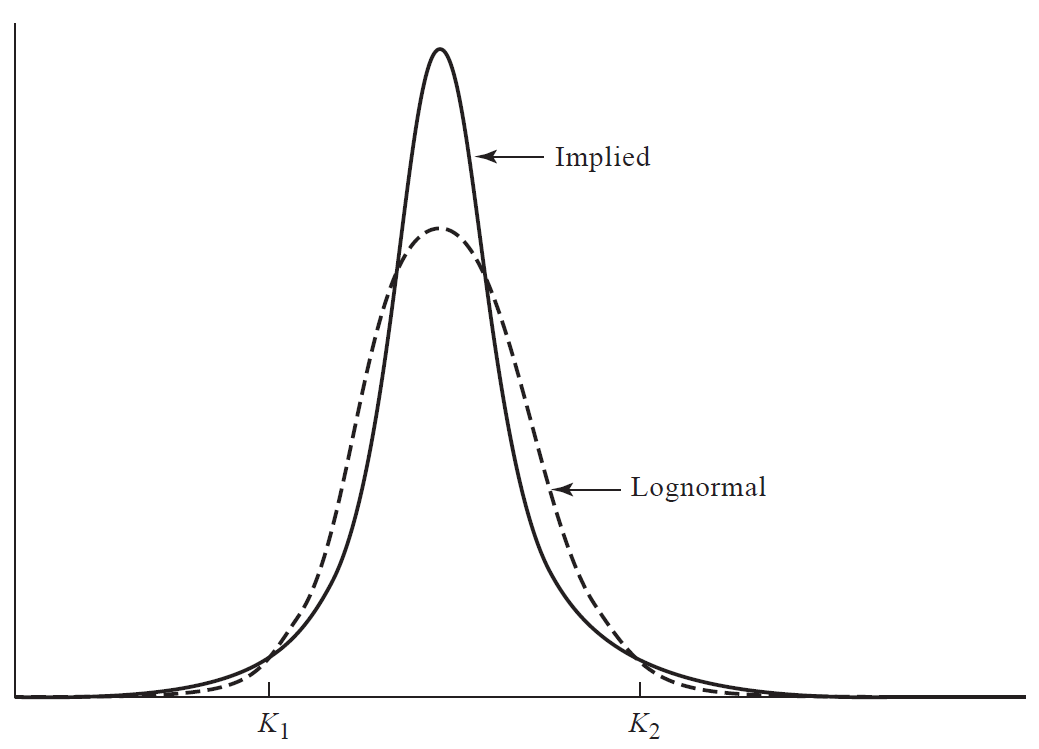
\includegraphics[width=.8\linewidth]{Media/currency_distribution.PNG}
  \caption{Foreign currency market}
%  \label{fig:sub1}
\end{subfigure}%
\begin{subfigure}{.5\textwidth}
  \centering
  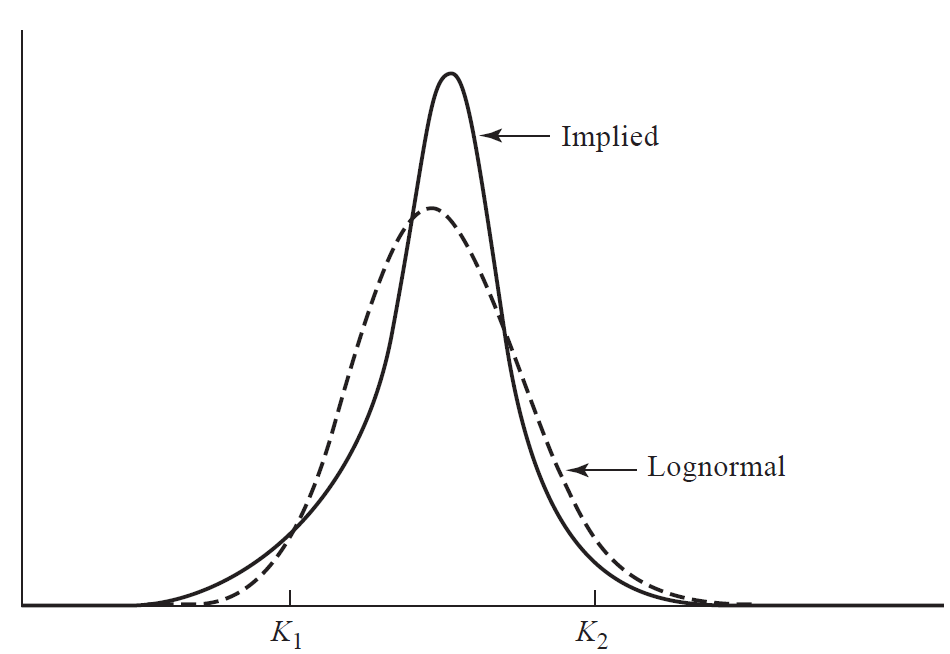
\includegraphics[width=.9\linewidth]{Media/equity_distribution.PNG}
  \caption{Equity market}
%  \label{fig:sub2}
\end{subfigure}
\caption{From \cite{hul09}. GBM (Lognormal) and Implied distributions for typical markets.}
\label{fig:implied_distribution}
\end{figure}

\section{Heston Model} \label{chap:heston_model}

The Black and Scholes model presented in section \ref{subsec:bs} fails to capture essential well-known properties of the real world market dynamics of the underlying return distributions, as its high kurtosis, its negative skew, the correlation between the underlying price and its volatility... As well as the risk premium investors give deep ITM or OTM options, which result in the volatility discussed in section \ref{subsec:smile_and_surf}.

To address that, several variations of this model have been proposed since it was introduced. Some of them, called stochastic volatility (SV) models, considered all the real world dynamics mentioned above and treated both the underlying price and its volatility as (potentially correlated) stochastic processes.

One of the first and most well-known SV models is the Heston model, defined by the following system of stochastic differential equations.

\begin{definition} Heston model price-volatility equations:
$$
dS_t = \mu S_t dt + \sqrt{\nu_t} S_t W_t^{(1)}
$$
$$
d\nu_t = \kappa(\overline{\nu} - \nu_t) dt + \sigma \sqrt{\nu_t}dW_t^{(2)}
$$
$$
dW_t^{(1)}dW_t^{(2)} = \rho dt
$$
, where $\nu_t$ is the variance of the underlying asset price at time t. The parameters $\kappa$, $\overline{\nu}, \sigma, \rho$ are respectively called: mean-reversion rate, long-term variance, volatility of volatility, and correlation between the Brownian processes $W_t^{(1)}$ and $W_t^{(2)}$. From now on, $\theta := (\nu_0, \overline{\nu}, \rho, \kappa, \sigma)$ will refer to the set of model parameters.
\end{definition}

Several studies have shown the relations between the Heston model parameters and the shape of the implied volatility surface \cite{cla11, gat06, gil12, jan11} necessary to obtain the same prices with a BS model. These relations can be summarized as follows:

\begin{itemize} \label{hes_param_properties}
\item $\nu_0$ controls the position of the volatility surface.
\item $\rho$ controls its skewness.
\item $\kappa$ and $\sigma$ control the convexity of the surface.
\item $\kappa(\nu_0 - \overline{\nu})$ controls the term structure of implied volatility.
\end{itemize}

Heston also provided an expression of the price of an European option, which will be adapted here in terms of the state variables x and y defined in section\ref{subsec:european_option_valuation}:

\begin{align} 
\label{eq:option_valuation_expectation}
& v(x, \tau) & = e^{-r \tau}\E^{\Q}(v(y, 0)|x) & = e^{-r \tau} \E^{Q}(K(e^y - 1)\boldsymbol{1}_{y \geq 0}) \\  
\label{eq:option_valuation_useless}
&  &  & = Ke^{-r \tau}(\E^{Q}(e^y \boldsymbol{1}_{y \geq 0}) - \E^{Q}(\boldsymbol{1}_{y \geq 0})) \\
\label{eq:option_valuation_final_form}
&  &  & = K e^x e^{-q \tau} P_1(\boldsymbol{\theta}; x, \tau) - K e^{-r \tau} P_2(\boldsymbol{\theta}; x, \tau)
\end{align}
, where $P_1$ and $P_2$ are defined as:
\begin{align}
&P_{1}(\boldsymbol{\theta} ; x, \tau)=\frac{1}{2}+\frac{1}{\pi} \int_{0}^{\infty} \operatorname{Re}\left(\frac{e^{i u x}}{i u} \frac{\phi(\boldsymbol{\theta} ; u-i, \tau)}{\phi(\boldsymbol{\theta} ;-i, \tau)}\right) \mathrm{d} u\\
&P_{2}(\boldsymbol{\theta} ; x, \tau)=\frac{1}{2}+\frac{1}{\pi} \int_{0}^{\infty} \operatorname{Re}\left(\frac{e^{iux}}{i u} \phi(\boldsymbol{\theta} ; u, \tau)\right) \mathrm{d} u
\end{align}
, where $\phi$ is the characteristic function of the process followed by the logarithm of price of the underlying asset. The expression of this characteristic function is
\begin{equation} \label{eq:char_heston}
\phi(\boldsymbol{\theta} ; u, \tau):=\mathrm{E}\left[\exp \left(i u \log \frac{S_{t}}{S_{0}}\right)\right]=\exp \left\{i u \log \frac{F}{S_{0}}\right.
\left.\quad+\frac{\kappa \bar{v}}{\sigma^{2}}\left[(\xi+d) \tau-2 \log \frac{1-g_{1} e^{d \tau}}{1-g_{1}}\right]+\frac{v_{0}}{\sigma^{2}}(\xi+d) \frac{1-e^{d \tau}}{1-g_{1} e^{d \tau}}\right\}
\end{equation}
, where $F := S_t e^{(r - q) \tau} = S_t \phi(\boldsymbol{\theta; u, \tau}$ is the forward price and

\noindent\begin{minipage}{.3\linewidth}
\begin{equation}
\xi:=\kappa-\sigma \rho i u
\end{equation}
\end{minipage}
\noindent\begin{minipage}{.4\linewidth}
\begin{equation} \label{eq:char_d}
d:=\sqrt{\xi^{2}+\sigma^{2}\left(u^{2}+i u\right)}
\end{equation}
\end{minipage}
\noindent\begin{minipage}{.3\linewidth}
\begin{equation}
g_{1}:=\frac{\xi+d}{\xi-d}
\end{equation}
\end{minipage}

Substituting these values into equation \ref{eq:option_valuation_final_form} , one can obtain an analytic equation to obtain the price of European Call options:

% TODO: Change all this to log(F/K) instead of log(K/F)

\begin{lem} Heston's pricing method.
\begin{equation} \label{eq:heston_analytic}
\begin{aligned}
C(\theta ; K, \tau)=& \frac{1}{2}\left(S_{t} e^{-q \tau}-K e^{-r \tau}\right) \\
&+\frac{e^{-r \tau}}{\pi}\left[S_{0} \int_{0}^{\infty} \operatorname{Re}\left(\frac{e^{-i u \log \frac{K}{S_0}}}{i u} \phi(\theta ; u-i, \tau)\right) \mathrm{d} u\right. \\
&\left.-K \int_{0}^{\infty} \operatorname{Re}\left(\frac{e^{-i u \log \frac{K}{S_0}}}{i u} \phi(\theta ; u, \tau)\right) \mathrm{d} u\right]
\end{aligned}
\end{equation}

% TODO: We should split it into the part that depends on the forward F_{t,T} and K, and the other one and explain that they are quite independent. When valuating, we assume the price of the forward to be S_0 * exp of whatever. Just look at gatheral's book.
% Also explain a bit that we assume the risk neutral drift to be r - q (though in our simulations we will set q = 0)
\end{lem}

From this expression, one can compute the analytic gradients of the option price in terms of the derivatives of the characteristic function. Then they can be used to optimize an appropriate objective function using gradient-descent based methods (See chapter \ref{chap:optimization_problem}) but, as will be explained in the next section, the analytic derivatives have not been widely used traditionally to calibrate Heston models prior to Cui et al. due to the complexity of the expressions obtained by derivating the available characteristic function expressions as eq \ref{eq:char_heston}  \cite{cui17}.

\subsection{Calibration Difficulties}
As opposed to simpler 1-dimensional models, Heston model calibrations is a multidimensional optimization problem with 5 degrees of freedom. Furthermore, the structure of this optimization problem is not known.

According to \cite{cui17} no consensus exists among researcher regarding whether the objective function of this optimization problem is convex or not. Some results point to a non-convex function, as the calibration methods proposed in \cite{che07, mik03} (which yielded different results for different initial points) and one must use long or short term approximations and rules to provide a sufficient initial guess. Recent research claims to provide methods that reach a unique solution independently of the initial point \cite{ger12} which, according to that study this indicates some structure that, even if not necessarily convex, tends to lead an initial guess to a stationary result.
There's also no consensus on whether the problem always has a single  optimum. In particular, it is known that there exists dependencies between the parameters that yield to similar results. For example, $lim_{t \rightarrow \infty} Var(\nu_t) = \dfrac{\sigma^2 \overline{\nu}}{\kappa}$, so large values of $\kappa$ and $\sigma$ can provide a model that prices options similarly to one with proportionally smaller values of these two parameters. The study by Cui et al. \cite{cui17} defends that this yields to the the objective function of the optimization problem flat close to the optimum.

As said above, there's no guarantee that a gradient-based method converges to the global optimum of the model parameters, but even obtaining a local optimum has been traditionally difficult. A lot of literature uses numerical gradients\cite{ger12} for these methods when trying to solve the Heston calibration problem (which are less accurate and more computationally consuming), because no simple analytic gradients were available and the ones obtained with symbolic algebra packages from the expressions of the characteristic function were intractable.

Prior to the work of Cui et al. \cite{cui17}, the existing methods could be summarized as:

\begin{itemize}
\item{\textbf{Heuristic based models:}}
Using the relationships stated in \ref{hes_param_properties}, some studies reduce the dimension of the optimization problem by assuming some values or relationships between the parameters from the observation of a specific volatility surface. For example, Gatheral sets $\nu_0$ to the short-term ATM implied variance obtained by using a BS model \cite{gat06}, an heuristic further justified by Chen \cite{che07}, where the linearity between $\nu_0$ and the BS implied volatility was verified for short maturities (less than 2 months). Other heuristics used in the industry are $\kappa = \dfrac{2.75}{\tau}$ and setting $\overline{\nu}$ to the BS short term volatility \cite{cla11}.

These assumptions may restrict the optimization problem domain and exclude the optimum.
2.2.2.
\item{\textbf{Stochastic methods:}}
They are usually used in combination with deterministic search methods, as the Nelder and Mead simplex method \cite{lag98} and would avoid the pitfalls of the gradient-based methods if the optimization problem is not convex. Some examples are Wang-Landau \cite{che07}, differential evolution and particle swarm \cite{gil12_2}, and simulated annealing \cite{moo09}.
These methods are too computationally expensive for real-time use as of now: Fernandez et al. use GPU computations to calibrate options using a SV model called SABR, and it took 421.72 seconds to calibrate 12 instruments with tolerance of $10^{-2}$ using 2 NVIDIA Geforce GTX470 GPUs \cite{fer13}.

\item{\textbf{Deterministic methods:}}

\end{itemize}

\subsection{Alternative Expressions}

For long-term maturities (i.e. big values of $\tau$), Kahl and J\"{a}ckel show that the characteristic  \ref{eq:char_heston} has discontinuities as $u$ increases \cite{kah06}, which can lead to numerical problems for many option valuation methods based on the integral expression \ref{eq:integral_option_valuation}. They show that this discontinuities arise because of a term in equation \ref{eq:char_heston} of the form $G^\alpha(u) := e^{\alpha log G(u)}$ with $G(u) := \dfrac{1 - g_1 e^{d\tau}}{1 - g_1}$ and $\alpha := \dfrac{\kappa \overline{\vega}}{\sigma^2}$, for non-integer values of $\alpha$. This is due to the spiral shape of $G(u)$ which produces a phase jump on $log(G(u))$ each time $G(u)$ crosses the negative side of the real line.

Albrecher et al. \cite{alb07} showed that the dicontinuity arises from taking the principal value of the square root in d (see equation \ref{eq:char_d}) and it can be avoided if the second value is used. In fact, it was proven that this alternative expression was continuous in the full parameters space \cite{sch04}

\begin{lem}
\begin{equation} \label{eq:char_schouten}
\phi(\boldsymbol{\theta} ; u, \tau)=\exp \left\{i u \log \frac{F}{S_{0}}
+\frac{\kappa \bar{v}}{\sigma^{2}}\left[(\xi-d) \tau-2 \log \frac{1-g_{2} e^{-d \tau}}{1-g_{2}}\right]+\frac{v_{0}}{\sigma^{2}}(\xi-d) \frac{1-e^{-d \tau}}{1-g_{2} e^{-d \tau}}\right\} 
\end{equation}
, where $g_2 = \dfrac{1}{g_1}$
\end{lem}

A more compact version of the characteristic function was later derived by del Ba\~no Rollin et al. \cite{rol10} from the moment generating function of the process. This expression also had the benefit of replacing the u-dependent power functions in equations \ref{eq:char_heston} and \ref{eq:char_schouten} by hyperbolic functions, which greatly simplified obtaining analytic expressions of the gradient of the characteristic function.

\begin{lem}
\begin{equation}
\phi(\boldsymbol{\theta} ; u, \tau)=\exp \left(i u \log \frac{F}{S_{0}}-\frac{\kappa \bar{v} \rho \tau i u}{\sigma}-A\right) B^{2 \kappa \bar{v} / \sigma^{2}}
\end{equation}

, where
\begin{equation}\begin{array}{l}
A:=\frac{A_{1}}{A_{2}} \\
A_{1}:=\left(u^{2}+i u\right) \sinh \frac{d \tau}{2} \\
A_{2}:=\frac{d}{v_{0}} \cosh \frac{d \tau}{2}+\frac{\xi}{v_{0}} \sinh \frac{d \tau}{2} \\
B:=\frac{d e^{\kappa \tau / 2}}{v_{0} A_{2}}
\end{array}\end{equation}
\end{lem}

This last expression also showed discontinuity problems, as the original characteristic function in equation\ref{eq:char_heston}, but Cui, del Ba\~no Rollin, and Germano provided an equivalent expression, continuous in the full parameters domain, and with an analytic expression for its gradient.

\begin{thm} \textbf{Cui's expression of the Heston characteristic function.}
\begin{equation}
\phi(\boldsymbol{\theta}; u, \tau) = exp \left(i u log \dfrac{F}{S_{0}}-\dfrac{\kappa \bar{v} \rho \tau i u}{\sigma}-A + \dfrac{2 \kappa \bar{v}}{\sigma^{2}}D \right)
\end{equation}
is an algebraically equivalent representation of equation \ref{eq:char_heston}, continuous through all the parameters space, where
\begin{equation}
D := \log \frac{d}{v_{0}}+\frac{(\kappa-d) \tau}{2}-\log \left(\frac{d+\xi}{2 v_{0}}+\frac{d-\xi}{2 v_{0}} e^{-d \tau}\right)
\end{equation}
. Further, its gradient with respect to the Heston model parameters $\boldsymbol{\theta} = (\nu_0, \overline{\nu}, \sigma, \kappa, \rho)^{T}$ is given by:
\begin{equation}
\nabla \phi(\boldsymbol{\theta}; u, \tau) = \boldsymbol{h}(u) \phi(\boldsymbol{\theta}; u, \tau)
\end{equation}
, where $\boldsymbol{h}(u) = [h_{v_0}(u), h_{\overline{v}}(u), h_\sigma(u), h_\kappa(u), h_\rho(u)]^T$ and:
\begin{align}
h_{v_0}(u)& =-\frac{A}{v_{0}} \\
h_{\overline{v}}(u)& =\frac{2 \kappa}{\sigma^{2}} D-\frac{\kappa \rho \tau i u}{\sigma} \\
h_{\sigma}(u)& =-\frac{\partial A}{\partial \rho}+\frac{2 \kappa \bar{v}}{\sigma^{2} d}\left(\frac{\partial d}{\partial \rho}-\frac{d}{A_{2}} \frac{\partial A_{2}}{\partial \rho}\right)-\frac{\kappa \bar{v} \tau i u}{\sigma} \\
h_{\kappa}(u)& =\frac{1}{\sigma i u} \frac{\partial A}{\partial \rho}+\frac{2 \bar{v}}{\sigma^{2}} D+\frac{2 \kappa \bar{v}}{\sigma^{2} B} \frac{\partial B}{\partial \kappa}-\frac{\bar{v} \rho \tau i u}{\sigma} \\
h_{\rho}(u)& =-\frac{\partial A}{\partial \sigma}-\frac{4 \kappa \bar{v}}{\sigma^{3}} D+\frac{2 \kappa \bar{v}}{\sigma^{2} d}\left(\frac{\partial d}{\partial \sigma}-\frac{d}{A_{2}} \frac{\partial A_{2}}{\partial \sigma}\right)+\frac{\kappa \bar{v} \rho \tau i u}{\sigma^{2}}
\end{align}

\end{thm}

\subsection{Moment Generating Function} \label{subsec:heston_moment}

In \cite{rol09}, the moment generating function for the Heston model is provided for the stochastic variable $X_t := ln(S_t) - \mu \tau$. Adapting it to provide it for $y|x$ one obtains:
\begin{equation}
\begin{aligned}
M(u)=\mathbb{E}\left[ e^{u X_{t}}\right] = e^{- x u} exp & \left[ \dfrac{2 \kappa \overline{\nu}}{\sigma^{2}} \left( \dfrac{(\kappa-\sigma \rho u) \tau}{2} - log \left(cosh \left(\dfrac{P(u) \tau}{2} \right)+(\kappa-\sigma \rho u) \dfrac{sinh \left(\dfrac{P(u) \tau}{2} \right)}{P(u)}\right) \right) \right. \\
& \left. -\mu \tau -v_{0} \dfrac{\left(u-u^{2}\right) \dfrac{sinh \left(\dfrac{P(u) \tau}{2} \right)}{P(u)}}{cosh \left(\dfrac{P(u) \tau}{2} \right)+(\kappa-\sigma \rho u) \dfrac{sinh \left(\dfrac{P(u) \tau}{2} \right)}{P(u)}} \right]
\end{aligned}
\end{equation}

, where $P(u)=\sqrt{(\kappa -\rho \sigma u)^{2}+\sigma^{2}\left(u-u^{2}\right)}$

This expression will be useful to bound the mass at the queues of the probability function $f(y|x)$.

\begin{lem} \label{lem:my_lemma}
\begin{equation}
C(\boldsymbol{\theta}; K, \tau) = Ke^{-r\tau} \left[ \dfrac{e^x - 1}{2} + \dfrac{1}{\pi} \int_0^{\infty} Re \left( \dfrac{\hat{f}(u - i; x) - \hat{f}(u; x)}{iu} \right) du \right]
\end{equation}
\end{lem}

\begin{lem} \label{lem:my_lemma_2}
\begin{equation}
C(\boldsymbol{\theta}; K, \tau) \approx C_1 :=  Ke^{-r\tau} \left[ \dfrac{e^x - 1}{2} + \dfrac{1}{\pi} \sum_{1 - \kappa}^{\kappa} D_{m,k} \int_0^{\infty} Re \left( \dfrac{\hat{\phi}_{m,k}(u - i) - \hat{\phi}_{m,k}(u)}{iu} \right) du \right]
\end{equation}
\end{lem}

\section{Multi Resolution Analysis and Shannon Wavelets}

\subsection{Multi Resolution Analysis} \label{def:mra}
Multi Resolution Analysis (MRA) is a method that ultimately allows to express any function in $L^2(\R)$ using a countable orthogonal family of wavelets. This family can then be truncated into a finite family and the original function can be orthogonally projected into the resulting subspace, obtaining an approximation with a certain level of resolution. Increasing the considered number of members of the wavelet family will increase the resolution of the approximation, converging to a perfect representation when all the wavelets are used \cite{tour}.

Given the space $L^2(\R) = \left\{f: \int_{-\infty}^{\infty}{|f(x)|^2 dx < \infty} \right\}$, a Multi Resolution Analysis is defined as 
a family of nested successive approximation closed spaces:
$$ \cdots \subset V_{-2} \subset V_{-1} \subset V_0 \subset V_1 \subset V_2 \subset \cdots $$

Where the subpsaces $V_i$ are complete (they are not redundant and cover $L^2(\R)$:
$$\overline{\bigcup_{i\in{\Z}}{V_i}} = L^2(\R) \text{, and } \bigcap_{m\in{\Z}} = {0}$$

, they have self-similarity in scale (all spaces are geometric scalings of $V_0$ by powers of 2):
$$ f(x) \in V_i \Leftrightarrow f(2x) \in V_{i + 1} $$

, they have self-similarity in time:
$$ f(x) \in V_0 \Rightarrow f(x - k) \in V_0, \forall k \in \Z $$

(Note that self-similarity in scale implies that the self-similarity in time translates to all spaces $V_i$ as $f(x) \in V_i \rightarrow f(x - 2^i k) \in V_i$.), and the integer shifts of a (or a finite group of) generator function $\phi$ form an orthogonal basis of $V_0$. 

In summary, we can define:

\begin{definition} \label{def:mra} (MRA): Consider $\phi \in L^2(\R)$ a wavelet that spans the family $\{\phi_{m,k}\}m,k\in\Z$ defined as the normalized scaled integer shifts of $\phi$. That is, $\phi_{m,k} = 2^{m/2}\phi(2^m x - k)$, and let $V_m := closure_{L^2(\R)}\left\langle\{\phi_{m,k}\}_{k \in \Z}\right\rangle$ 
\end{definition}

Then, if $\phi$ and $V_m$ fulfill the conditions above, we say that $\phi$ is the scaling function or father wavelet of the MRA $\{V_m\}$ (note that the previous definition properly defines $\{V_m\}$ as a sequence of nested subspaces and that $\phi$ provides an orthonormal basis for each of them).

One of the important implications of obtaining a father wavelet and its MRA is that another wavelet family can be obtained from it, which will be a basis of $L^2(\R)$. In order to do that, let's consider the set of subspaces $W_m$ such that $V_{m+1} = V_m \oplus W_m$. Then $L^2(\R) = \sum_m{\oplus W_m}$ and there exists a function $\psi \in W_0$ (called mother wavelet) that generates an orthonormal basis of $L^2(\R)$ \cite{dau92} by defining the wavelet functions:
$$ \psi_{m, k} = 2^{m/2}\psi(2^m x - k)$$
. Note that each $\{W_{m,k}\}_{k \in \Z}$ gives an orthonormal basis of $W_m$, and $\{W_{m_k}\}_{m\in [-\infty, m-1], k \in \Z}$ is an orthonormal basis of $V_m$. So for any $m \in \Z$ we can define 
\begin{definition} \label{def:wavelet_projection}
\textbf{Wavelet Projection:} $P_m: L^2(\R) \rightarrow V_m$ is the projection from any function $f \in L^2(\R)$ into $V_m$:
\begin{equation} 
P_m f(x) = \sum_{j = -\infty}^{m-1} \sum_{k \in \Z} d_{j,k} \psi_{j, k}(x) = \sum_{k \in \Z} D_{m,k} \phi_{m, k}(x)
\end{equation}

, where $d_{j, k} = \left\langle f,\psi_{j, k}\right\rangle$, $D_{m,k} = \left\langle f,\phi_{m, k}\right\rangle$, and $\left\langle f,g\right\rangle = \int_\R f(x) \overline{g(x)} dx$. Further, this projection converges in the $L^2$ norm as m tends to infinity \cite{tour}.
\end{definition}

\subsection{Shannon Wavelets}
Claude Shannon introduced the usage of the cardinal sine function for information modeling \cite{sha49}:
\begin{equation}
sinc(x) := \left\{ \begin{array}{rcl} \dfrac{sin(\pi x)}{\pi x} & \mbox{for} & x \neq 0 \\ 1 & \mbox{for} & x = 0 \end{array}\right.
\end{equation}

This function serves as the father wavelet from which we obtain the families $\phi_{m, k}$ and $\psi_{m_k}$:
\begin{equation}
\begin{array}{rcl}
\phi_{m,k}(x) = 2^{m/2} sinc(\pi (2^m x - k)), & k \in \Z
\end{array}
\end{equation}
\begin{equation}
\begin{array}{rcl}
\psi_{m,k}(x) = 2^{m/2} \left( sinc(\pi (2^m x - k - 1/2)) - \dfrac{sin(2 \pi (2^m x - k - 1/2))}{\pi (2^m x - k - 1/2)} \right), & k \in \Z
\end{array}
\end{equation}

One of the interesting properties of Shannon wavelets it that they have both a slow decay in time domain and a simple expression and sharp compact support in the frequency domain.
\begin{equation} \label{eq:sharp_freq}
\begin{array}{rcl}
\hat{\phi}_{m,k}(w) = \dfrac{e^{-i k/2^m w}}{2^{m/2}}rect \left(\dfrac{w}{2^{m+1}\pi}\right), & k \in \Z
\end{array}
\end{equation}
\begin{equation}
\begin{array}{rcl}
\hat{\psi}_{m,k}(w) = -\dfrac{e^{-i \dfrac{k + 1/2}{2^m} w}}{2^{m/2}} \left(rect \left(\dfrac{w}{2^{m}\pi} - \dfrac{3}{2}\right) + rect \left(-\dfrac{w}{2^{m}\pi} - \dfrac{3}{2}\right) \right), & k \in \Z
\end{array}
\end{equation}

When using Shannon Wavelets to approximate a function with a truncated wavelet expansion \cite{mar17} shows a bound for the projection error into $V_m$, by using concepts of band-limited functions:

\begin{definition} A function f is called band-limited if $\exists B \in \R^+$, with $B < \infty$ such that
\begin{equation}
f(x) = \dfrac{1}{2\pi} \int_{-B \pi}^{B \pi} \hat{f}(u) e^{iu x}du 
\end{equation}
, that is, the support of $\hat{f}$ is contained in the interval $[-B, B]$. The parameter B is referred to as the bandwidth of f.
\end{definition}

The nested subspaces of a Shannon MRA can be expressed in terms of band-limited functions because of the sinc Fourier transform rectangular shape, as stated in the following lemma from \cite{ste11}

\begin{lem} Consider an MRA generated from the Shannon scaling function as defined in \ref{def:mra}, then each subspace $V_m$ corresponds to the space of functions $f \in L^2(\R)$ with bandwidth $B \leq 2^m$
\end{lem}

Combining this lemma with the $L^2$ convergence of the projections $P_m$ of $f$ into $V_m$ yields the following corollary \cite{mar17}

\begin{cor} The orthogonal projection $P_m$ of a Shannon MRA is equivalent to:
\begin{equation}
P_m f(x) = \dfrac{1}{2 \pi} \int_{-2^m \pi}^{2^m \pi} \hat{f}(u) e^{i u x} d u
\end{equation}
\end{cor}

Which, in turn, can be used to derive the following bound to the error of the orthogonal projection.

\begin{definition}Given $f \in L^2(\R)$, let $H(\xi)$ be:
\begin{equation}
H(\xi) := \dfrac{1}{2 \pi} \int_{|u| > \xi}\left|\hat{f}(u)\right| du
\end{equation}
, the normalized mass of the two-side tails of $\hat{f}$ defined by $\xi$.
\end{definition}

\begin{lem} \label{lem:projection_error} Let $\epsilon_m(x) := f(x) - P_m f(x)$ (the pointwise approximation error due to the projection of f into $V_m$). Then $|\epsilon_m(x)| \leq H(2^m \pi)$ \cite{mar17}
\end{lem}


\subsection{Sinc Integral}\label{sec:sinc_integral}
Shannon MRA and SWIFT require solving integrals of the form $\int_{\R} f(x) g(sinc(x)) dx$. In particular, when one wants to compute the density coefficients $D_{m,k}$ of equation \ref{def:wavelet_projection}, or as will be seen in section \ref{subsec:payoff_coefficients}, for the payoff coefficients computation, one needs to solve integrals of the form $\int_{\R} f(x) \overline{\phi(x)} dx$ and $\int_{\R} f(x) \phi(x) dx$ respectively.

The simplest situation is to compute the sinc integral $Si(t) = \int_0^t{sinc(x) dx}$, but even for this case there is no closed form for the integral. 

There are two commonly used approaches as to how to numerically approximate these integrals, and their equivalency wa. 

\begin{itemize}
\item{ \textbf{Coefficients via Parseval's Theorem: } This approach, shown in \cite{ort16} uses the fact that the $\phi_{m,k}$ has a very small support in the frequency domain (as shown in equation \ref{eq:sharp_freq}) together with Parseval's theorem, 
$\langle f, g \rangle = \dfrac{1}{2 \pi}\langle \hat{f}, \hat{g} \rangle$. As the coefficients will be real numbers, we can take $\langle f, g \rangle = Re \left( \langle f, g \rangle \right) = Re \left( \dfrac{1}{2 \pi}\langle \hat{f}, \hat{g} \rangle \right)$. Entering the real part operator inside the integral sign and applying the change of variable $t = \dfrac{u}{2^{m+1} \pi}$ results in expression:
\begin{equation}
D_{m,k} = 2^{m/2} \int_{-1/2}^{1/2} Re \left(\hat{f}(2^{m+1} \pi t) e^{i2\pi k t} \right) dt
\end{equation} 
Any quadrature can be applied to numerically compute the integral, but there are known techniques to rearrange the trapezoid and midpoint quadratures to compute all the coefficients with a single FFT \cite{mar17, flo20}.
}
\item { \textbf{Coefficients via Sinc approximations: }
An equivalent expression of the sinc function was presented in \cite{ort16} as a cosine expansion using Vieta's formula: 
\begin{equation}
sinc(x) = \prod_{j = 1}^{\infty} cos \left( \dfrac{\pi x}{r^j} \right)
\end{equation}
This cosine expansion was then truncated and converted to a summation via the cosine product-to-sum-identity
\begin{equation} \label{eq:density_v}
\prod_{j=1}^{\iota} \cos \left(\frac{\pi x}{2^{j}}\right)=\frac{1}{2^{\iota-1}} \sum_{j=1}^{2^{\iota-1}} \cos \left(\frac{2 j-1}{2^{\iota}} \pi x\right)
\end{equation}
obtaining the first expression for the vieta coefficients $D_{m,k}^v$, where
\begin{equation}
D_{m,k} \approx D_{m,k}^{v}= \frac{2^{m / 2}}{2^{\iota-1}} \sum_{j=1}^{2^{\iota-1}} \int_{\mathbb{R}} f(x) \cos \left(\frac{2 j-1}{2^{\iota}} \pi\left(2^{m} x-k\right)\right) d x
\end{equation} \label{eq:density_vc}
Finally, $f(x)$ would be replaced in the integral by defining $D_{m,k}^{v} = Re \left( D_{m,k}^{vc} \right)$. 
\begin{equation}
D_{m,k}^{vc} =  \dfrac{2^{m / 2}}{2^{\iota-1}} \sum_{j=1}^{2^{\iota-1}} \int_{\mathbb{R}} f(x) e^{-i\dfrac{2 j-1}{2^{\iota}} \pi\left(2^{m} x-k\right) } d x
\end{equation}
Notice that when applying the $Re(\cdot)$ operator to $D_{m,k}^{cv}$, it can move freely across multiplications by real numbers and sumations and integrals, and expression \ref{eq:density_v} is ultimately recovered by using $Re \left(e^{-uix}\right) = cos(x)$. Finally, splitting the complex exponential into x-dependent and x-independent terms and replacing $\int_{\R} f(x) e^{-xAi}$ by $\hat{f}(A)$ yields:
\begin{definition} \textbf{Vieta coefficients approximation}\label{def:vieta}
\begin{equation}
D_{m,k}^{*} =  \dfrac{2^{m / 2}}{2^{\iota-1}} \sum_{j=1}^{2^{\iota-1}} Re \left( \hat{f} \left(u_j 2^{m} \right) e^{ik u_j} \right)
\end{equation}
, where $u_j = \dfrac{\pi}{2^{\iota}}(2j - 1)$
\end{definition}
}
\end{itemize} 

It is worth noting that, while the original construction of expression \ref{def:vieta} required a sumation of a power of 2 number of terms, it was revisited in \cite{mar17} and generalized by expressing the sinc in terms of its Fourier transform 
\begin{equation}
sinc(t) = Re(sinc(t) = \dfrac{1}{2\pi} \int_{-\pi}^{\pi} Re \left( e^{-iux} du \right) = \dfrac{1}{\pi} \int_{0}^{\pi} cos(ux) du
\end{equation}
Then, if one uses a mid-point quadrature with J buckets and proceeds as in the initial derivation, expression \ref{def:vieta} is recovered, with the new term J being equivalent to the previous $2^{\iota -1}$ one.

The following approximation error bound was given in \cite{mar17} for the mid-point quadrature, which will be of special interest in section when analysing the approximation error of pricing an option with the SWIFT algorithm in section \ref{subsec:approximation_error}:

\begin{lem} \textbf{Error of the Sinc Integral Approximation}
\begin{equation} \label{lem:error_sinc}
sinc(x) \approx sinc^{*}(x; J) = \dfrac{1}{J}\sum_{j = 1}^J Re\left( e^{-iu_jx} \right)
\end{equation}
, where $u_j = \dfrac{\pi (2j - 1)}{2J}$. Then the approximation error of applying the midpoint quadrature on a finite domain $|x| \leq a \leq \dfrac{\pi}{2}J$ is bounded by:
\begin{equation}
max_{|x| \leq a} \left|sinc(x) - sinc^{*}(x; J) \right| \leq \dfrac{(\pi a)^2}{(4J)^2 - (\pi a)^2}
\end{equation}
\end{lem}

\section{Pricing by Gatheral}

\section{SWIFT}

The Shannon Wavelets Inverse Fourier Technique (SWIFT) combines the Shannon Wavelets and Multiresolution Analysis concepts with equation \ref{eq:integral_option_valuation} to provide a fast approximation to the value of a specific option v(x, t).

The overall approximation can be summarized, as in \cite{mar17}, by a set of consecutive approximation steps to that equation, which are described below. The error related to each of these approximations will be analyzed in section \ref{subsec:approximation_error}.

\begin{itemize} \label{swift_steps}

\item \textbf{Wavelet Projection:} f is substituted by its Shannon wavelet projection at scale $m \in \Z$. By lemma \ref{def:wavelet_projection} this can be stated as:
\begin{equation} \label{step:wavelet_projection}
f(y|x) \approx f_1(y|x) := P_mf(y|x) = \sum_{k \in \Z} D_{m,k}(x) \phi_{m,k}(y)
\end{equation}
\begin{equation}
v(x,t) \approx v_1(x,t) = e^{-r \tau} \int_{\R} f_1(y|x)v(y, T)dy
\end{equation}
, with $D_{m,k}(x):=\langle f(\cdot | x), \phi_{m,k} \rangle$
\item \textbf{Series Truncation: } The set of values of k partaking the sum \ref{step:wavelet_projection} is reduced to a finite interval $[k1, k2]$
\begin{equation}
f_1(y|x) \approx f_2(y|x) = \sum_{k = k1}^{k2} D_{m,k}(x)\phi_{m,k}(y)
\end{equation}
\begin{equation} \label{step:series_truncation}
v_1(x,t) \approx v_2(x,t) = e^{-r \tau} \int_{\R} f_2(y|x)v(y, T)dy
\end{equation}
It is important to notice that the first approximation lets us express: 
\begin{equation}
f(2^{-m}k|x) \approx f_1(2^{-m}k|x) = 2^{m/2} D_{m,k}(x)
\end{equation}
, which quickly justifies that, for any given x, the density coefficients vanish as $|k|$ increases, because f vanishes at the queues. It is also worth noting that increasing m will result in this mapping being less favorable. That is, for each k, $D_{m,k}$ will be bounded by a point closer to the center of the density function, potentially requiring to increase the interval $[k1, k2]$.
\begin{remark}
From this point onward a symmetric interval $[1 - \kappa, \kappa]$ will be considered both for convenience and for consistency with the code implementation.
\end{remark}
\item \textbf{Density Coefficients Approximation: }
The integral required to compute $D_{m,k}$ is replaced by an approximation $D_{m,k}^{*}$ as discussed in section \ref{sec:sinc_integral}.
\begin{equation}
f_2 (y|x) \approx f_3(y | x) = \sum_{k = 1 - \kappa}^{\kappa} D_{m,k}^{*}(x)\phi_{m,k}(y)
\end{equation}
\begin{equation}
\begin{aligned}
v_2(x,t) \approx v_3(x,t) & = e^{-r \tau} \int_{\R} f_3(y|x)v(y, T)dy \\
&= e^{-r \tau} \sum_{k = 1 - \kappa}^{\kappa} D_{m,k}^{*}(x)  V_{m,k}dy
\end{aligned}
\end{equation}
, where
\begin{equation}
V_{m,k} := \int_{\R} \phi_{m,k}(y) v(y, T)dy
\end{equation}
\item \textbf{Payoff Coefficients Approximation: }
The integral required to compute $V_{m,k}$ is approximated in an analogous way as the integral to compute the density coefficients.
\begin{equation}
v_3(x,t) \approx v_4(x,t) = e^{-r \tau} \sum_{k = 1 - \kappa}^{\kappa} D_{m,k}^{*}(x) V_{m,k}^{*}
\end{equation}

For European Put options the payoff is given by equation \ref{eq:european_payoff}, and the last equation can be rearranged using the strike-free payoff as

\begin{equation}
v_4(x,t) = K e^{-r \tau} \sum_{k = 1 - \kappa}^{\kappa} D_{m,k}^{*}(x) U_{m,k}^{*}
\end{equation}
, where $U_{m,k}^{*}$ is the approximation of 
\begin{equation} \label{eq:compact_payoffs}
U_{m,k} := \int_{\R} \phi_{m,k}(y)g(y) dy = \int_{-\infty}^{0} \phi_{m,k}(y)(1-e^{y}) dy
\end{equation}

This coefficients can be precomputed when initializing the SWIFT procedure and shared across different strikes and maturities, saving computation time.
\begin{remark}
The approximation $D_{m,k}^{*}$ depends on a parameter J that represents the number of intervals in the sinc approximation quadrature. The parameter used for payoff computation is independent from the one used for the density coefficients, and will be labeled $J_p$ and $J_d$ respectively.
\end{remark}
\end{itemize}

\begin{remark}
This section and section \ref{subsec:approximation_error} follow closely section 3 of \cite{mar17}. There, the error analysis of the approximation process starts with a truncation of the integration space of equation  \ref{eq:integral_option_valuation}, for which an explicit error bound is not provided. Here, this error is accounted for in the payoff coefficients approximation step and its explicitly specified.
\end{remark}

\subsection{Payoff Coefficients Approximation} \label{subsec:payoff_coefficients}
One should note that the same procedure as the approximation $D_{m,k} \approx D_{m,k}^{*}$ (discussed in section \ref{sec:sinc_integral}) can be used for the payoff coefficients approximation. Starting from expression \ref{eq:compact_payoffs}, and applying the same sinc approximation as in the density coefficients, for european puts we obtain expression:

\begin{equation}
U_{m,k} \approx \dfrac{2^{m/2}}{J_p}\sum_{j=1}^{J} e^{i \dfrac{2j - 1}{N_p} \pi k} \int_{\R} (1 - e^x)^{+} e^{-i \dfrac{2j - 1}{N_p} \pi x}
\end{equation}

The last step of the density coefficients approximation requires the convergence of the Fourier transform of the payoff coefficients which, in general, is not guaranteed. In particular the Fourier transform of the strike-free payoff of an european put option can only be described by the use of generalized functions:
\begin{lem} The Fourier transform of the strike-free Europan put payoff is given by:
\begin{equation}
\int_{\R} (1 - e^x)^{+} e^{- i u x} dx = \int_{-\infty}^{0} (1 - e^x) e^{- i u x} dx = \dfrac{i}{u} + \delta(u) - \dfrac{i}{u + i}
\end{equation}
, where $\delta(u)$ is the Dirac delta distribution.
\begin{proof}

\begin{equation}
\int_{\R} (1 - e^x)^{+} e^{- i u x} dx = \int_{-\infty}^{0} (1 - e^x) e^{- i u x} dx = 
\end{equation}
\end{proof}
\end{lem}

Typically, the SWITF algorithm implementations deal with this situation by initially bounding integral \ref{eq:integral_option_valuation} to a finite interval. Here, for simplicity a symmetric interval (-c, c) will be considered, reaching expression:

\begin{definition} \textbf{Strike-free payoff coefficients approximation}
\begin{equation}
U_{m,k} \approx U_{m,k}^{*}(-c, c) := \dfrac{2^{m/2}}{J_p}\sum_{j=1}^{J_p} Re \left(e^{i \dfrac{2j - 1}{N_p} \pi k} I_{j}(c)\right)
\end{equation}
, where
\begin{equation}
I_{j}(c) := \int_{|y| \leq c} g(y) e^{-i \dfrac{2j - 1}{N_p} \pi y} dy
\end{equation}
And its analytic expression can be easily computed for European options and is provided in appendix \ref{app:payoff_integral}.
\end{definition}

One can easily see that the value of $I(c)$ will be periodic on c. In general, all the sinc approximations used in the SWIFT algorithm are periodic, which can give rise to boundary issues and undervaluation of option prices when the option strikes approach the boundary of $(-c, c)$. This issue also appears in the COS option pricing method \cite{Fang2008}, another Fourier-transform-based option pricing method closely rleated to the SWIFT method, and is discussed by Maree et al. \cite{mar17}. In their study, they use the independence between the parameters regulating the payoff integral domain (c) and the one regulating the wavelet series truncation ($\kappa$) to carefully choose a value for c to avoid this problem.

\subsection{Fast Computation of the Density and Payoff Coefficients}
Starting with a general expression of the sumation term that appears in both the density and payoff coefficient approximation:
\begin{equation}
f_k = \sum_{j=1}^J g_j e^{i \dfrac{2j - 1}{2J}\pi k}
\end{equation}
One can extend it by defining $g_j = 0$ for $j = 0$ and $J < j < 2J$ and take the j-independent terms outside of the sumation, obtaining:
\begin{equation}
f_k = e^{\dfrac{-i \pi k}{2J}}\sum_{j=0}^{2J - 1} g_j e^{i \dfrac{2j\pi k}{2J}}
\end{equation}

This last sumation expression coincides with the Discrete Fourier Transform (DFT) of length 2J of $\{g_j\}$, and the computation of all the values $f_k$ can then be sped up by using a Fast Fourier Transform (FFT) implementation. 

\begin{remark}
Note that computing the density or payoff coefficients imposes a restriction on the wavelet series truncation parameter $2 \kappa < J$
\end{remark}

In all numeric examples in this article the C library FFTW will be used to compute any FFT.

\subsection{Alternative Method for Multiple Strikes}


If one were to use the SWIFT pricing 
A great property of the SWIFT method is that it allows to reuse most of its calculations to price several strikes for L\'evy and Heston models

Change the strike dependency from the density to the payoff coefficients

\begin{lem} Option Price
\begin{equation}
v(\boldsymbol{\theta}; x, \tau) \approx v_1(\boldsymbol{\theta}; x, \tau) = e^{-r \tau} \int_{I_m} v(y, 0) f_m(\boldsymbol{\theta}; y|x) dy = e^{-r \tau} \sum_{k = k_1}^{k_2} D_{m,k}(\boldsymbol{\theta}; x) \cdot V_{m, k}
\end{equation}
, where $$V_{m, k} = \int_{I_m} v(y, 0) \phi_{m,k}(y)dy$$
\end{lem}

\subsection{Option Price Gradient}

The SWIFT option pricing scheme will be used to calibrate different models by using an optimization problem, as described in chapter \ref{chap:optimization_problem}. For gradient-based optimization methods, the gradient of the pricing formula used will be required. Thus, one needs to compute the gradient of $v_4(\boldsymbol{\theta}; x, \tau)$

\begin{lem} Option Price Gradient
\begin{equation}
\nabla_{\boldsymbol{\theta}} v_4(\boldsymbol{\theta}; x, \tau) = e^{-r \tau} \sum_{k = k_1}^{k_2} V_{m, k}^{*} \nabla_{\boldsymbol{\theta}} D_{m,k}^{*}(\boldsymbol{\theta}; x)
\end{equation}
with
\begin{equation}
\nabla_{\boldsymbol{\theta}} D_{m,k}^{*} (\boldsymbol{\theta}; x) = \dfrac{2^{m/2}}{2^{J-1} \sum_{j=1}^{2^{J-1}}} Re \left[ 
\nabla_{\boldsymbol{\theta}} \hat{f}\left(\boldsymbol{\theta}; x, \dfrac{(2j - 1) \pi 2^m}{2^J}\right) e^{\dfrac{ik\pi(2j-1)}{2^J}}\right] 
\end{equation}
\begin{proof}

\end{proof}
\end{lem}

\subsection{Approximation Error Analysis and SWIFT Parameter Choice} \label{subsec:approximation_error}

\begin{itemize}
\item \textbf{Integration Range Truncation: }
\begin{equation}
\epsilon_{0} := 
\left| v_0(\boldsymbol{\theta}; x, \tau) - v(\boldsymbol{\theta}; x, \tau) \right| = 
\int_{|y| > c} 
f(y|x) v(y, \tau) 
dy \leq \tau(c) ||v(y, \tau)||_{\infty}
\end{equation}
For European put options $ ||v(y, \tau)||_{\infty} = ||K (1 - e^y)||_{\infty} = K $, so the error can be made arbitrarily small.
\item \textbf{Wavelet Projection:}
A bound for $\epsilon_m := f(y|x) - P_mf(y|x)$ is provided in lemma \ref{lem:error_sinc}. An approximation to this bound, which converges exponentially with respect to $2^m$ is presented in \cite{mar17} for several L\'evy functions which, for the GBM process is given by:
\begin{equation}
\epsilon_m \approx \dfrac{(2^m \pi)^{-1}}{4 \pi \tau}\left( \left| \hat{f}(-2^m;x) \right| + \left| \hat{f}(2^m;x)\right| \right)
\end{equation}

TODO: Heston

This provides an iterative method to try increasing values of m until the error $\epsilon_m$ falls under a desired threshold.

\item \textbf{Series Truncation: }



\item \textbf{Density Coefficients Approximation: }

Lemma \ref{lem:error_sinc} immediately allows to bound the error of approximating the Shannon wavelets by using $sinc^{*}$:
\begin{cor} \label{cor:error_shannon_wavelets} \textbf{Shannon Wavelet Approximation Error:}
For a fixed $J \geq \dfrac{\pi}{2}(2^m c + k)$
\begin{equation}
max_{|y| \leq c, 1 - \kappa \leq k \leq \kappa} \left| \phi_{m,k}(y) - \phi^{*}_{m,k}(y) \right| \leq 2^{m/2}\dfrac{(\pi(2^m c + \kappa))^2}{(4J)^2 - (\pi(2^m c + \kappa))^2}
\end{equation}
\end{cor}
\item \textbf{Payoff Coefficients Approximation: }

\begin{equation}
\tau(c):= \int_{|y| > c} f(y|x) dy \leq TOL
\end{equation}

\end{itemize}

\begin{equation}
D_{m,k}(\boldsymbol{\theta}; x) \approx c^*_{m,k} (\boldsymbol{\theta}; x) = \dfrac{2^{m/2}}{2^{J-1}} \sum_{j=1}^{2^{J-1}} \R \left[\hat{f}\left(\boldsymbol{\theta}; x, \dfrac{(2j - 1) \pi 2^m}{2^J}\right) e^{\dfrac{ik\pi(2j-1)}{2^J}}\right] 
\end{equation}

As shown in \cite{ort16}, one can take the set $\{X_{m,k}\}$

\subsection{Swift Parameters Choice}

\section{Calibration as an optimization problem} \label{chap:optimization_problem}
The goal of calibrating a model using market data, is to obtain model parameters that, when used for option valuation with an appropriate option valuation method, yield results similar to the real market option prices.

Completely matching the market for all strikes and maturities is an over-determined problem so, generally, the calibration consists on a least squares minimization problem, using a set of option market prices at different strikes and maturities.

In this section, the objective function of the optimization problem used by \cite{cui17} is presented, as it will be the one used in this study.

\subsection{Objective Function}
Let $C^*(K_i, \tau_i)$ be the market price of a European call option and
 $C(\boldsymbol{\theta}; K_i, \tau_i)$ be the price at the same strikes and maturities obtained by using the Heston analytic formula \ref{eq:heston_analytic}. Let's also assume that we use n different options to calibrate the model, so 
 $i \in [1,n] \subset \Z$
 . Then:
 \begin{definition} The calibration of the model is defined as the minimization problem $$min_{\boldsymbol{\theta} \in \R^5} (f(\boldsymbol{\theta}))$$ $$f(\boldsymbol{\theta}) := \dfrac{1}{2}||\boldsymbol{r}(\theta)||^2 = \dfrac{1}{2} \boldsymbol{r}^T(\boldsymbol{\theta})\boldsymbol{r}(\boldsymbol{\theta})$$
\end{definition}

, where $\boldsymbol{r}(\boldsymbol{\theta})$ is the n-dimensional vector of the residuals obtained when pricing the options considered for calibration using the model parameters. That is:

\begin{align}
\boldsymbol{r}(\boldsymbol{\theta}) := \left[r_1(\boldsymbol{\theta}), \ldots, r_n(\boldsymbol{\theta}) \right]^T, 
&& r_i(\boldsymbol{\theta}) :=  C(\boldsymbol{\theta}; K_i, \tau_i) - C^*(K_i, \tau_i), && i = 1, \ldots, n
\end{align}

It is worth noting that the choice of a specific objective function (and appropriate strikes and maturities to use as calibration points) will intimately characterize the model. This can be used when trading to fit to the specific needs of trader, ultimately leading to different objective functions, as relative price differences instead of absolute ones, or log-likelihood based methods \cite{jac00} for, for example, hedging and market making \cite{chr02}. 

One must be cautious, as this choice can lead to consistently giving more weight in the calibration to some set of options over the others. For example, according to \cite{cui17}, a commonly used minimization problem in industry for calibration consists on a least-squares problem similar to the one used in this study, using squared differences of the implied BS volatility of each calibration option, which can lead to giving more weight to OTM options in comparison with ITM ones.

The choice of calibration strikes and maturities can also have a similar impact in the pricing model. For example, as an option gets closer to the expiration date, the variance of the price change until expiration of the underlying asset gets smaller. So, if one were to always use the same strikes across different expiries, then for long-term maturities the model would end up with a lot of calibration points ATM but would lack control points in regions where the density function of the underlying asset is still relevant, which could lead to serious pricing errors for mildly OTM and ITM options. For the short-term maturities, the relevant regions of the density function would have small number of sparse strikes and there would be a lot of strikes in very OTM and ITM regions, where prices are mostly close to 0 and to the discounted payout respectively, so they are less sensitive to the change in the model parameters and do not help much in calibration (the price derivatives with respect to the model parameters will be almost flat at those expiry-maturity points, so they will not affect much the optimization problem), effectively wasting computational power.

As this study does not strive for any specific trading strategy, the choice of TODO: finish this and mention that the calibration objective function should be the same as the one used when valuating the model performance \cite{chr02}

%% Anava per aqui1

\section{Gradient Calculation} \label{sec:gradient}

\begin{equation}
\begin{aligned}
\nabla C(\boldsymbol{\theta} ; K, \tau)=\frac{e^{-r \tau}}{\pi} &\left[\int_{0}^{\infty} \operatorname{Re}\left(\frac{e^{-i u \log \frac{K}{s_{0}}}}{i u} \nabla \phi(\boldsymbol{\theta} ; u-i, \tau)\right) \mathrm{d} u\right.\\
-&\left.K \int_{0}^{\infty} \operatorname{Re}\left(\frac{e^{-i u \log \frac{K}{s_{0}}}}{i u} \nabla \phi(\boldsymbol{\theta} ; u, \tau)\right) \mathrm{d} u\right]
\end{aligned}
\end{equation}
, where 

\subsubsection{Fast Calculation of integrands}
All integrands are of the form: % PAGE 6, right column.

\section{Formulation of the study}

In this study a Heston model will be calibrated with a a Levenberg–Marquardt method with the objective function defined in \ref{eq:objective_function}. 

The option valuation will be done with a SWIFT method, using the expression for the characteristic function and it's derivatives provided in \cite{cui17}. These derivatives are taken from an exact expression of the option price. In order for the difference between the real derivatives and the derivatives of the Shannon Wavelet approximation to be small, the approximation error will be restricted accordingly.

\subsection{Pricer Stress Tests}
Both the option pricing presented by Cui, using the Gatheral equations \cite{cui17} and the SWIFT

\subsection{Robustness and general minima tests} \label{test:robustness}
There is no guarantee the objective function of the calibration problem is convex, so local minima problems can arise so, in order to both validate the robustness of the method proposed and assert its region of attraction, several convergence tests will be run.

Consider a set of initial parameter configurations $\{\boldsymbol{\theta}^*\}$. Given an initial parameter vector $\boldsymbol{\theta}_{i}^*$ its correspondent call option prices will be computed at 40 control points $C(K_j, \tau_j)$.

These points will be combination of 8 expiries at expiries (TODO: add expiries when they are decided) (to take into account both short-term and long-term maturities) and 8 strikes taken at 0\%, $\pm 25 \% $, and $\pm 50 \%$ BS delta, as recommended in section \ref{sec:optimization_problem} (TODO: make sure it's explained there). Then, random perturbations will be applied to each initial parameters vector to obtain a set of transformed parameters
$\{\boldsymbol{\theta}_i\}$. The proposed calibration methodology will then be applied to these parameters and the convergence region and local optimization minimums will be studied.


\subsection{Speed tests}
The SWIFT approach with all its speed-up techniques should improve the computation time with respect to the original option valuation method used in the study of Cui et al. \cite{cui17}, and this speed-up should. In order to quantify this speed improvement several sets of Heston model parameters and market parameters (at both long and short term expiries and OTM and ITM options, to provide an heterogeneous sample of contracts) will be generated. For these inputs, the price of their correspondent option price will be computed using both the swift method and a simple quadrature numerical integration as in \cite{cui17}.

\subsection{Fit tests}
The Heston model should capture the market dynamics like skewness and high-kurtosis better than other simpler models like Black and Scholes. In particular, it should be able to capture the volatility smile for a given expiry. The only way to observe this phenomenon is through the use of real market data.

As said in section \ref{subsec:smile_and_surf}, important market events, like the 1987 Black Monday, can affect the implied volatility smile. The Covid-19 pandemic we are currently under has affected q

In order to illustrate reasons a simple comparison between BS and Heston with real market data from EMini S\&P 500 options will be included. The calibration points will be obtained from real market data and will be taken for a single expiry at 

The value goodness-of-fit 

Christoffersen and Jacobs \cite{chr02} show the importance of using the same objective function for both model calibration and goodness-of-fit tests, and to use the same one across the different models we want to compare. This will not 

Comparing directly the goodness-of-fit of a Heston model and a BS one should show the clear dominance of the first one.

\section{Numerical Results}

\subsection{Numerical Issues With Regular Cui Method}

TODO: Check why Cui failed so horribly

\section{Conclusions}

\begin{itemize}

\item \textbf{Robustness}

Cui doesn't provide how to set the integration boundary. The method runs into numerical errors when u is too big, so a far-off initial guess of option parameters won't converge if N is not dynamically set. If it is, we would need to take it into account when computing the gradient. In summary, this limits the region of attraction of the method.

SWIFT provides a dynamic scheme to set the pricing parameters, so one doesn't run into that kind of issue. On the other hand, if one decides to change the pricer parameters while running the gradient descent, one would need to to compute the total derivatives with respect to the option parameters by taking into account how changing the heston parameters changes the swift parameters and then how the swift parameters change the option parameters. Some of the parameters change discretely, so everything would be discontinuous.

Another possibility would be to bound the error between the heston gradient and the real option price gradient. If the parameters are chosen so that the heston gradient is close enough to the heston price gradient through all the domain, and the price is also bounded, then every step of the gradient descent would take as closer to the optimum, if the real gradient is not too flat.

\item \textbf{Speed}

\item \textbf{Fitness}

\end{itemize}

\section{Further Research}
Heston model clearly shows an improved fit with respect to the BS one, but this improvement could be mainly explained by the fact that BS has only 1 model parameter while Heston has 5.

In order to give a fair comparison between both models, it would be of to also compare the performance of a hybrid BS model that can deal with the volatility smile to some extent. This model would be defined by 5 BS volatilities $\boldsymbol{\sigma} = (\sigma_1, \sigma_2, \sigma_3, \sigma_4, \sigma_5)$, computed at specific control points in the delta space (for example at $\pm50\%$, $\pm25\%$, and $0\%$ delta, like in the original fitness test). Then, the volatility at any delta would be defined by an interpolation scheme, like natural splines.

\section{Bibliography}

%\newpage

\bibliography{biblio}{}
\bibliographystyle{plain}

%______________________________________________________________
\appendix
\vfill\newpage 
\section{Code}
The implementation of the SWIFT coded for this work can be consulted in the following Github public repository:


\section{Expressions}

\subsection{Strike-free European Options Payoff Integrals} \label{app:payoff_integral}

\subsection{Trapezoid Quadrature For Parseval Coefficients}

\end{document}